\slajdid{06-s018}
\begin{frame}[label=06-s018]{Binarni kod – promena dve sukcesivne vrednosti – 8 u 7, 1000 u 0111}
\gusttekst\begin{columns}[c,onlytextwidth]
\column{.235\textwidth}\centering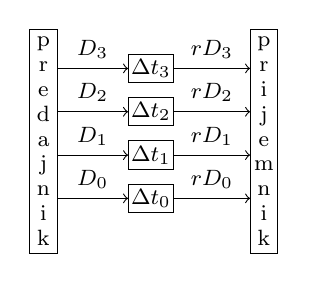
\begin{tikzpicture}[x=1cm,y=1cm,font=\fontsize{8}{9}\selectfont]
\draw (0,-.2) rectangle (.35,2.65);\node[align=center] at (.175,1.225) {p\\r\\e\\d\\a\\j\\n\\i\\k};
\draw (2.8,-.2) rectangle (3.15,2.65);\node[align=center] at (2.975,1.225) {p\\r\\i\\j\\e\\m\\n\\i\\k};
\draw[->] (.35,2.15)--(1.25,2.15) node[midway,above] {$D_3$};
\draw (1.25,1.97) rectangle (1.83,2.33);\node at (1.54,2.15) {$\Delta t_3$};
\draw[->] (1.83,2.15)--(2.8,2.15) node[midway,above] {$rD_3$};
\draw[->] (.35,1.5999999999999999)--(1.25,1.5999999999999999) node[midway,above] {$D_2$};
\draw (1.25,1.42) rectangle (1.83,1.7799999999999998);\node at (1.54,1.5999999999999999) {$\Delta t_2$};
\draw[->] (1.83,1.5999999999999999)--(2.8,1.5999999999999999) node[midway,above] {$rD_2$};
\draw[->] (.35,1.0499999999999998)--(1.25,1.0499999999999998) node[midway,above] {$D_1$};
\draw (1.25,0.8699999999999999) rectangle (1.83,1.2299999999999998);\node at (1.54,1.0499999999999998) {$\Delta t_1$};
\draw[->] (1.83,1.0499999999999998)--(2.8,1.0499999999999998) node[midway,above] {$rD_1$};
\draw[->] (.35,0.4999999999999998)--(1.25,0.4999999999999998) node[midway,above] {$D_0$};
\draw (1.25,0.3199999999999998) rectangle (1.83,0.6799999999999997);\node at (1.54,0.4999999999999998) {$\Delta t_0$};
\draw[->] (1.83,0.4999999999999998)--(2.8,0.4999999999999998) node[midway,above] {$rD_0$};
\end{tikzpicture}

\column{.37\textwidth}\centering\input{slike/tikz/s018_vremenski_dijagram.tex}
\column{.36\textwidth}Zbog različitih kašnjenja, a menjaju se sva četiri bita, prijemnik može očitati pogrešne vrednosti, ako čita u „neodgovarajućim“ vremenima.\par\vspace{4mm}
1.\quad 1001 vrednost porasla umesto da opada\\2.\quad 1111 greška jako velika\\3.\quad Tek sada je prava
\end{columns}
\end{frame}
